%!TEX TS-program = xelatex
%!TEX encoding = UTF-8 Unicode

\def \papersize {a4paper}
\documentclass[12pt,\papersize]{extarticle}
% extarticle is like article but can handle 8pt, 9pt, 10pt, 11pt, 12pt, 14pt, 17pt, and 20pt text

\def \ititle {Mindreading and Joint Action: Philosophical Tools}
\def \isubtitle {Notes for Lecture 2}
\def \iauthor {Stephen A. Butterfill}
\def \iemail{ButterfillS@ceu.hu}
%for anonymous submisison
%\def \iauthor {}
%\def \iemail{}
%\date{}

\input{$HOME/Documents/submissions/preamble_steve_paper2}

%avoid overhang
\tolerance=5000


\begin{document}

\setlength\footnotesep{1em}

\bibliographystyle{newapa} %apalike

%these two lines are for anonymous submission --- they remove author and date
%but don't forget to remove defs above as well --- otherwise it will be in the metadata
%\author{}
%\date{}


\maketitle
%\tableofcontents
%
%\begin{abstract}
%\noindent
%***
%\ 
%
%\noindent
%\textbf{Keywords:}
%Mindreading, Joint Action, Action, Belief, Intention, Representation, Mental State
%\end{abstract}
%



\section{Terminology}


\textit{Mindreading} is 
	the process of 
	identifying mental states and actions 
	as the mental states and actions of a particular subject 
	on the basis, ultimately, of bodily movements and their absence,
somewhat as reading is the process of identifying propositions on the basis of inscriptions \citep[p.\ 4]{Apperly:2010kx}.


\section{Slide}
Last week I suggested that we don’t adequately understand what mindreading is.
Of course we can *define* mindreading.
Mindreading is the process of identifying mental states and actions as the mental states and actions of a particular subject on the basis, ultimately, of bodily movements and their absence, somewhat as reading is the process of identifying propositions on the basis of inscriptions (Apperly 2010, p. 4).
Not adequately understanding mindreading means that there are questions we can’t answer, and puzzles we can’t resolve, and that a deeper understanding of what mindreading is might be needed to answer those questions and resolve those puzzles.
Anyway, this week I start from the assumption that we agree on wanting a deeper understanding of what mindreading is.
As mindreading is defined in terms of mental states, the natural question to ask is,
What are mental states?

Need to be careful here.  Since our interest is in mindreading, we don’t necessarily want the truth about mental states.  We merely want a theoretically coherent conception of them.


\section{Slide}
To illustrate the need for this, consider Call \& Tomasello’s claim.
What are Call \& Tomasello saying the chimps understand?


\section{Slide}
First note that this is a claim about understanding.  They are not saying that chimps discriminate situations in which another knows from situations in which she is ignorant.
They are saying that chimps understand something about the knowledge states that constitute the difference between these situations.



\section{Slide}
But what are they saying when they say that chimps understand knowledge?  What does this amount to?


\section{Slide}
Take Quassim Cassam ... are they saying that Chimpanzees have this conception of knowledge? Probably not.  After all, they may not want to be committed to saying that chimpanzees think of knowledge states as standing in need of explanation; they may not want to claim that chimpanzees sometimes think to themselves, I wonder how she knew about that?
But then what conception of knowledge do Call \& Tomasello think chimpanzees have?

I think that this quote is fine if it is intended just to give us a very rough idea about what chimpanzees think.
But it would be a mistake to think that it gives us deep insight into what chimpanzees represent that enables them to track knowledge states.
The problem is that, pre-theoretically, we don’t have a clear enough sense of what ‘knowledge’ is to know what might be involved in understanding knowledge.

My aim in asking what mental states are is this.
If we can characterise---or mischaracterise---knowledge, belief and others, then we might be in a position to be more explicit about what chimpanzees and humans and others understand


\section{Slide}

\begin{center}
  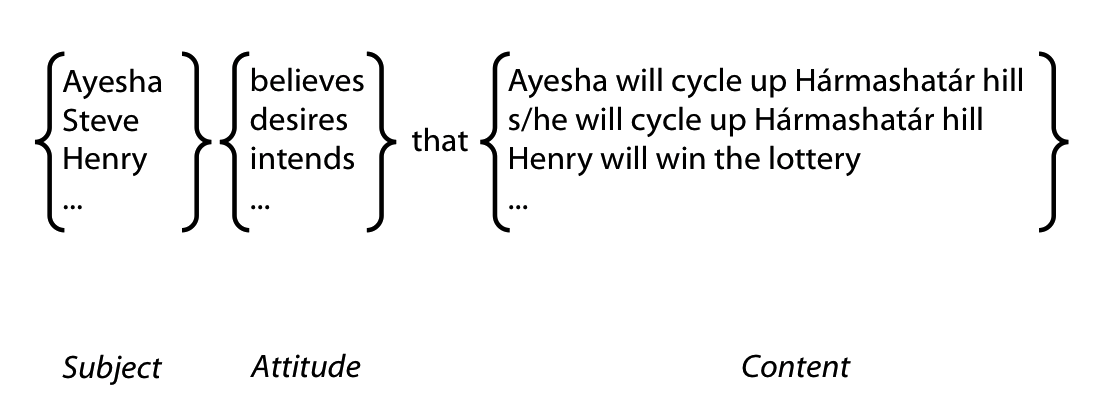
\includegraphics[width=0.3\textwidth]{fig4n.png}
\end{center}

The content is what distinguishes one belief from all others, or one desire from all others.
The content is also what determines whether a belief is true or false, and whether a desire is satisfied or unsatisfied.

There are two main tasks in constructing a theory of mental states. 
The first task is to characterise the different attitudes.
This typically involves specifying their distinctive functional and normative roles.
The second task is to find a scheme for specifying the contents of mental states.

Let’s start with the second task and come back to the first.  [***OR SHOULD I POSTPONE THE SECOND TASK UNTIL THE LECTURE ON MEASUREMENT?]


\section{Slide}
The second task is to find a scheme for specifying the contents of mental states.
Usually this is done with propositions.
But what are propositions?
Propositions are abstract objects like numbers.
They have more mystique than numbers, but, like numbers, they are abstract objects that can be constructed using sets plus a few other basic ingredients such as objects, properties and possible worlds.



\section{Slide}
There are actually quite a few different views about what propositions are.
For example, McGrath says that ‘Propositions ... are the sharable objects of the attitudes and the primary bearers of truth and falsity’ \citep{McGrath:2012pro}.

Others introduce propositions by appeal to sentences, or utterances of sentences.  Here the idea is that a proposition is what the utterance of a sentence expresses and that in virtue of which the utterance is true or false (as well as that in virtue of which it is necessary, if it is necessary). \citep{King:2011pro}





\section{Slide}
We can remain agnostic about these ideas and think about propositions simply as abstract objects like numbers.

Just as there are different kinds of number---natural, rational and real, for instance---there are also different kinds of proposition.

And just as one way to get a handle on what numbers are is to see how they can be constructed from more basic ingredients, like sets, so equally one way to get a handle on propositions is to see how they can be constructed from ingredients we are already familiar with.

Propositions are abstract objects like numbers.
They have more mystique than numbers, but, like numbers, they are abstract objects that can be constructed using sets plus a few other basic ingredients such as objects, properties and possible worlds.


\section{Slide}
I’m about to explain how to construct propositions.
But you might ask why we are bothering.
We already have abstract objects, namely sentences.
Why not just use sentences to specify the contents of mental states?
That’s only because sentences are not suitable for this purpose.
We want a collection of abstract objects that we can use to specify the contents of mental states; so, ideally, we would set things up so that there is only one belief corresponding to each abstract object.
And sentences don’t have this property.
Take the sentence, "s/he will cycle up Hármashatár hill”
This sentence refers to different desires depending on who the subject is.
(What I desire when I cycle up the hill is different from what you desire when you desire that you cycle up the hill; after all, one of these desires might be satisfied while the other is not.)
So we can’t use sentences to specify the contents of mental states because some sentences are associated with indefinitely many different beliefs.
Instead we need a collection of abstract object such that we can associate at most one belief associated with each object.

You might think we could get around this by avoiding using sentences that contain ‘she’ and other indexicals.
But John Perry has shown that this is impossible.
The problem in a nutshell is that Ayesha’s desire that she cycle up the hill is different from her desire that Ayesha cycle up the hill because even though she is Ayesha, she might not know that.

You might think something must have gone wrong here.
We use utterances of sentences to identify what someone believes or desires all the time. 
After all, I can tell you what someone desires like this: "Mo desires that s/he will cycle up Hármashatár hill".
So how can I be saying that we can’t use sentences to distinguish the contents of mental states?
The answer is simple.
When we utter a sentence we express a proposition.
And it is the proposition, not the sentence, that we use to specify the content of a belief or desire or other mental state.

So there is no getting away from propositions.
But they’re also not particularly mysterious either.


\section{Slide}
But there is a second problem [with Singular Propositions].  Suppose Steve = Ayesha.  Then these are the same propositions.  But someone might have different beliefs. ... This is Oedipus and Jocasta ... which became te story of Heinz and his rubber in the work of Liz Robinson and Ian Apperly ... It’s impossible for these propositions to cut more finely than there are individuals in the world.  But it seems that mental states can cut more finely.  So perhaps we need a third kind of proposition.


\section{Slide}
Third type of proposition gets around all these problems.
So with the third type of proposition we have found a scheme for specifying the contents of mental states that seems to allow us to make as many distinctions as human adults intuitively make.

What can we conclude so far about representing mental states?
Someone who represents mental states needs some system of abstract objects, such as some kind of proposition, in order to have a way of distinguishing among their contents.
This doesn’t mean that they have to represent Fregean propositions: after all, they might represent mental states without being able to specify every possible difference in content.
So I’m not suggesting that anyone who represents mental states must be able to represent Fregean propositions.
The point is rather just that we understand what sort of thing is required ... and how different abstract objects that could be used to distinguish among the contents of mental states impose different limits.

[***Next issue: relation between beliefs and propositions --- are propositions *objects* of belief or are they simply measuring devices?
I will come back to this issue in Lecture 3 (on measuring, tracking and representing beliefs).]


\section{Slide}
So let’s return to Call \& Tomasello. 
Our first question in being more precise about their proposal is: What sort of abstract object do chimpanzees use to specify the contents of mental states (for example, to distinguish one intention from another)?
In the next lecture I’m going to compare attributing mental states to measuring temperature.
If you think chimpanzees can measure temperature, it makes sense to ask what sort of units they use to measure temperature.  E.g. do they use numbers or some other kind of scale?
Similarly, if we think chimpanzees can measure mental states, we can ask what sort of abstract objects they use to do this.
And, as we saw, different answers have different consequences for the limits of their abilities to represent mental states.  
So there is even some hope that different hypotheses about which abstract objects chimpanzees use might generate testable predictions.


\section{Slide}
.... and of course we have to ask the same question about infants and adults.
And we should maybe not take for granted that chimpanzees, infants and adults all use the same system of abstract objects to distinguish the contents of mental states.


\section{Slide}
Now to the other task ... how to characterise the attitudes?  


\section{Slide}
Now we can go back and ask whether these norms are part of different subjects’ understandings of the attitudes ...
But this hardly seems like a good question to ask.
What evidence might persuade us either way?

So I think there are two problems.
One is that there is no obvious basis for accepting or rejecting these claims about the attitudes.
The other is that this way of distinguishing the attitudes doesn’t seem to generate useful questions about mindreaders.

Fortunately there is a different approach, one that relies less on commonsense.
We want to get a sense of the space of possibilities ... of the different understandings one might have of intention, say.

Proposal: we should take a constructive approach---creature construction.
And we should have a model of the attitudes, one that is clearly enough explained that we can tell whether it is capable of explaining a given individual’s behaviour in a particular case.


\section{Slide}
Proposal: we should take a constructive approach---creature construction.
And we should have a model of the attitudes, one that is clearly enough explained that we can tell whether it is capable of explaining a given individual’s behaviour in a particular case.

The point of creature construction is to ensure coherence.  We want to have a functioning, viable creature at each stage.  You can’t just take a fish and throw in feet.  Having feet goes with certain kinds of limb structure and capacities for movement.

Where Call and Tomasello says chimps understand intentions but not beliefs, a reasonable question to ask is, what sort of creature has intentions but not beliefs.  By attempting to construct the creature we would get a clearer idea of how, on their view, the chimpanzee understands minds.  I’m not going to try that here, although I will offer a suggestion along these lines.  Instead today I want to start in the middle, with the most sophisticated creature that we can construct using a well-understood model.

***Davidson quote is relevant here (about nothing in between), but I used that last week

[Decided to go straight for decision theory as a point in the middle, rather than starting with mere goals, adding in states that modulate and then gradually working towards decision theory.]


\section{Actions, outcomes and conditions}
That was a bit abstract.
Let's get into details.
(What follows is based on \citealp{Jeffrey:1983oe}; it's not my own work.) 
I'm going to go very slowly at the start. 
This will be a bit painful if you're already familiar with decision theory, but it's worth it because we will use the basic ideas more than once.
(This will be important again in the context of joint action.)

Imagine we are deciding between two \emph{actions}, cycling to the seminar or catching the bus. 
Let's also suppose that we are only interested in two types of \emph{outcome} these actions could have, staying dry versus not staying dry and getting exercise versus not getting exercise.
Among the various possible outcomes, our preference ranking is:
%
\begin{enumerate}
\item getting exercise and staying dry
\item not getting exercise and staying dry
\item getting exercise and not staying dry
\end{enumerate}
%
Suppose we know that cycling will result in the third outcome, 3, whereas getting the bus will result in the second outcome, 2. 
Then we should get the bus.
In this situation, actions guarantee outcomes so how we act should depend just on which outcome we prefer.

Very often actions are not so simply linked to outcomes.
We often don't know whether we will get wet if we cycle.
Whether we get wet depends on further \emph{conditions}, such as whether it rains or whether there is flooding.
In general, which outcome occurs depends both on the actions we choose and on the conditions we encounter.


\begin{table}[htbp]
\begin{center}
\footnotesize	%shrink for better spacing
\begin{tabular*}{1\textwidth}{@{\extracolsep{\fill}} l c *{3}{cc} } 

\toprule

& \multicolumn{2}{c}{\emph{condition}} 
\\ 
\cmidrule(r){2-3}

 \emph{action} & no flooding & flooding
%
\\ \midrule
%
cycle & get exercise and stay dry & get exercise and get wet
\\
take bus & get no exercise and stay dry & get no exercise and stay dry 
\\
%
\bottomrule
%
\end{tabular*}
\caption{Outcomes depend on actions and conditions}
\end{center}	%careful -- position of this affects distance between table and caption(!)
\end{table}



Usually we are not certain about all the conditions relevant to a decision.
Instead we have to form a view about their probability.
For example, we might know that there is a fair chance of flooding without knowing outright that there is flooding.
This means we don't know for sure which outcome cycling will result in.
It might result in our most preferred outcome, getting exercise and staying dry; but it might also result in our least preferred outcome, getting exercise and getting wet.

For this reason, in deciding what to do we should ideally take into account both our preferences concerning the outcomes and  the probabilities of the conditions obtaining.
This could be done as follows.

We first consider the probabilities (see table \vref{table:probabilities}).
The top left cell represents the probability of no flooding if we choose to cycle.
%nb: if we choose to cycle, not *given that* we choose to cycle.  See http://plato.stanford.edu/entries/decision-causal/
Of course, the probability of flooding is independent of whether we cycle or take the bus.
But the approach is flexible enough to accommodate cases where our actions can influence the probability of the conditions ocurring.

\begin{table}[htbp]
\begin{center}
\footnotesize	%shrink for better spacing
\begin{tabular*}{1\textwidth}{@{\extracolsep{\fill}} l c *{3}{cc} } 

\toprule

& \multicolumn{2}{c}{\emph{condition}} 
\\ 
\cmidrule(r){2-3}

 \emph{action} & no flooding & flooding
%
\\ \midrule
%
cycle 
	& \begin{tabular}{c} 
		probability of 
		\\ no flooding if we cycle: 0.3 
	\end{tabular}
	& \begin{tabular}{c} 
		probability of 
		\\ flooding if we cycle:  0.7
	\end{tabular}
\\
take bus 
	& \begin{tabular}{c} 
		probability of 
		\\ no flooding if we get the bus: 0.3 
	\end{tabular}
	& \begin{tabular}{c} 
		probability of 
		\\ flooding if we get the bus: 0.7
	\end{tabular}
\\
%
\bottomrule
%
\end{tabular*}
\caption{Probabilities of four conditions obtaining}
\label{table:probabilities}
\end{center}	%careful -- position of this affects distance between table and caption(!)
\end{table}

We then assign weights to the outcomes that reflect how desirable they are in relation to each other (see table \vref{table:desirabilities}).

\begin{table}[htbp]
\begin{center}
\footnotesize	%shrink for better spacing
\begin{tabular*}{1\textwidth}{@{\extracolsep{\fill}} l c *{3}{cc} } 

\toprule

& \multicolumn{2}{c}{\emph{condition}} 
\\ 
\cmidrule(r){2-3}

 \emph{action} & no flooding & flooding
%
\\ \midrule
%
cycle 
	& \begin{tabular}{c} 
		[get exercise and stay dry] 
		\\ desirability of outcome: 3 
	\end{tabular}
	& \begin{tabular}{c} 
		[get exercise and get wet]
		\\ desirability of outcome:  -1
	\end{tabular}
\\
take bus 
	& \begin{tabular}{c} 
		[get no exercise and stay dry] 
		\\ desirability of outcome: 1 
	\end{tabular}
	& \begin{tabular}{c} 
		[get no exercise and stay dry] 
		\\ desirability of outcome:  1
	\end{tabular}
\\
%
\bottomrule
%
\end{tabular*}
\caption{Desirabilities of four outcomes}
\label{table:desirabilities}
\end{center}	%careful -- position of this affects distance between table and caption(!)
\end{table}


Finally we multiply the probability and desirability matrices (see table \vref{table:utilities}).
Adding the rows then gives expected utilities for each action.
The idea is that we should perform the act with the greatest expected utility.
In this case, cycling gets just 0.2 whereas taking the bus gets 1, so we should take the bus.

\begin{table}[htbp]
\begin{center}
\footnotesize	%shrink for better spacing
\begin{tabular*}{1\textwidth}{@{\extracolsep{\fill}} l c *{3}{cc} } 

\toprule

& \multicolumn{2}{c}{\emph{condition}} 
\\ 
\cmidrule(r){2-3}

 \emph{action} & no flooding & flooding
%
\\ \midrule
%
cycle & 0.3 [probability] $*$ 3 [desirability] = 0.9 & 0.7 $*$ -1 = -0.7
\\
take bus &   0.3 $*$ 1 = 0.3 &  0.7 $*$ 1 = 0.7
\\
%
\bottomrule
%
\end{tabular*}
\caption{Multiplying probabilities by desirabilities}
\label{table:utilities}
\end{center}	%careful -- position of this affects distance between table and caption(!)
\end{table}

I've gone very slowly over some familiar ideas because I want us to attend to the basics.
There are three basic elements: actions, conditions and outcomes.
Which outcome occurs depends on two things: the action chosen and the conditions that obtain.
Desirabilities attach to outcomes.
Probabilities attach to conditions.
Expected utilities attach to actions.
Expected utilities can be derived from desirabilities and probabilities.
One procedure for choosing an action is to compute expected utilities (in the way illustrated) and then perform the action with the highest expected utility.


\section{Reversing direction}
For simplicity I have so far been speaking as if we wanted to introduce a procedure for deciding how to act.
But of course that isn't our aim at all.
Our ultimate aim is to be able to justify  claims about attitudes---or at least to understand what sort of considerations might provide justification.
We still have a way to go.

So far we have seen how subjective probabilities and desirabilities determine expected utilities for actions.
If we knew the expected utilities of the actions available to an agent, we could make a prediction about how she will act---about whether she will cycle or take the bus, say.
But to work out an agent's expected utilities we would need to know the probabilities she assigns to relevant conditions and how desirable she finds the various outcomes.
How could we know this?
\textbf{What is the evidential basis for ascribing an agent subjective probabilities and desirabilities and how does the evidence support the ascriptions?}

Suppose we knew these things:
\begin{enumerate}
\item The agent will always perform an action with at least as much expected utility as any other actions available to her.
\item The agent has just two actions available to her: she can either cycle or get the bus.
\item The agent is getting the bus.
\end{enumerate}
Then we also know that the agent assigns the same, or higher, expected utility to getting the bus than to cycling.
So given some assumptions, an agent's actions reveal her expected utilities.

But this doesn't reveal much about the agent's preferences or probabilities.  
After all, expected utility is a function of both.
The agent might be getting the bus because she does not particularly desire exercise.
Or the agent might be getting the bus \emph{despite} particularly desiring exercise because she assigns a high probability to flooding (and a low desirability to staying dry).

On the face of it then, an agent's actions might reveal at most her expected utilities (given assumptions listed above) and leave us blind to her subjective probabilities and desirabilities.

If we knew the agent's subjective probabilities then, given some assumptions, we could work out her desirabilities from her expected utilities.
Someone who thinks flooding is likely but nevertheless cycles when she could have taken the bus must desire exercise more than staying dry. 




***HERE
*** intuitive explanation of Ramsey's criterion.



\subsection{Ramsey's insight}
Ramsey's criterion:
\begin{quote}
`Suppose that A and B are consequences [outcomes] between which the agent is not indifferent, and that N is an ethically neutral condition [i.e.\ the agent is indifferent between N and not N]. 
%strictly:  p 46: A con- dition is ethically neutral in relation to a particular agent and a particular consequence if the agent is indifferent between having that consequence when the condition holds and when it fails.
Then N has probability 1/2 if and only if the agent is indifferent between the following two gambles.
	\\ \hspace*{10 mm} B if N, A if not 
	\\ \hspace*{10 mm} A if N, B if not'
	\citep[p.\ 47]{Jeffrey:1983oe}
\end{quote}



\section{Slide}
 Want a method for determining subjective probabilities and subjective desirabilities from actions ... this ensures that the postulated states are knowable ... don’t have to have any way of measuring them independently, merely have to observe the decisions (assuming some background conditions are met, e.g. that the preferences are transitive)

\section{Slide}
There are lots of good objections to the idea that decision theory is a complete model of human behaviour ... one of these concerns joint action and in the Sugden paper, another concerns intention and is the topic of a later lecture.
The virtue of the decision-theoretic model is not that it is *right* but that it is clear enough to have limits.


\section{Slide}
This is what is missing from the account so far ... it focuses on the way desire and belief lead to action, ignoring the issue of how beliefs are acquired.

In other words: so far we have a theory of how attitudes relate to action but we do not have a theory about how they are acquired (a theory of belief fixation).
\begin{quote}
`A theory of mind needs a story about mental processes, not just a story about mental states. ... the logical behaviourism of Wittgenstein and Ryle had, as far as I can tell, no theory of thinking at all (except, maybe, the silly theory that thinking is talking to oneself). I do find that shocking. How could they have expected to get it right about belief and the like without getting it right about belief fixation and the like?' \citep[p.\ 9--10]{Fodor:1998ap}
\end{quote}
\begin{quote}
`modern philosophers ... have no theory of thought to speak of. I do think this is appalling; how can you seriously hope for a good account of belief if you have no account of belief fixation?' 
\citep[p.\ 147]{Fodor:1987rt}
\end{quote}



\section{Slide}
So the task was how to characterise the attitudes? 
Decision theory gives us a way of identifying attitudes like desire and belief without appeal to complexities like normative role.
But, unfortunately, it probably isn’t adequate as a theory of what these attitudes are, and it doesn’t straightforward give us an account of other attitudes like intending or loving.
So it is probably not a good model for explaining all of human action ... probably our mental lives are more complex than this allows.
But of course this doesn’t mean that it wouldn’t be a good model of the attitudes for a mindreader to adopt.



\section{Slide}
So we can imagine models of the attitudes that capture more complex than decision theory
And perhaps we can also develop models that capture even less complexity than decision theory as well.
These models could be taken as describing creatures with more and less sophisticated mental lives.

\section{Slide}
So when it comes to chimpanzees, we can ask two things about their understanding of mental states.  First, what is their model of the attitudes; and, second, what sort of scheme to they use for distinguish attitudes with different contents?  
The same goes for infant humans, and for adult humans as well.
After all, it’s a familiar idea that our thinking about the physical world might involve a variety of different models.
In lots of cases we can use a Newtonian theory as our working model of the world, or perhaps an even simpler one.
Just because we have discovered quantum mechanics doesn’t mean that we always have to use it.
When it comes to mindreading, I guess we’re sometimes more like engineers than scientists.
We want the simplest model that will give us results accurate enough for our purposes.

Another consequence of this view is that we shouldn’t assume that there is a massive chasm between abilities to think about behaviour and abilities to think about mental states.
After all, the process of applying a simple form of decision theory does not seem to require conceptual sophistication: anything from large-scale organisations to sensory-motor systems appear capable of implementing bayesian decision theory \citep{kording:2006_bayesian}.  So it is not a huge stretch to suppose that relatively primitive, automatic mechanisms might provide an implementation that is used not for determining how to act oneself but for predicting others’ actions.
It may be, then, that abilities to represent mental states are quite widespread.


\section{Slide: four questions}
Now let’s return to the questions I posed last lecture as indicators that we don’t adequately understand mindreading


\section{Slide: self-awareness}
This now seems quite straightforward.  Mastery of decision theory and ability to apply it to others seems no more connected to awareness of oneself as subject to the same laws than mastery of newtonian physics would require one to think of oneself as a physical object.  It seems conceiveable that could be individuals who thought about the physical world without realising that one was oneself a physical object ...


\section{Slide: evidence}
This question is answered by Ramsey’s insight ... essentially the evidence is choice actions ...


\section{Slide: holism}
Here we struggle.  We should try to find some way to do this.  But the natural way to proceed is to think of intention and knowledge as built on belief, as states involving more sophistication.  So this would be like saying that there could be mindreaders (chimpanzees) who can think about force but not mass or acceleration.


\section{Slide: objectivity}
I think the answer is yes ... but that is quite a long story.


\section{Slide}



\section{[***move] What is subjective desirability?  What is subjective probability?}
So far I have also not said what the desirabilities and probabilities are.
You may have some intuitions about what these represent.
In particular,  you may notice that they are intuitively related to desires and beliefs.
But strictly speaking so far we should treat as unresolved the issue of what these desirabilities and probabilities are.
Our aim is to use the desirabilities and probabilities to elucidate attitudes like belief and desire.
So it would clearly be a mistake to rely on those attitudes in saying what desirabilities and probabilities are.



%
%
%\section{What are mental states?}
%
%mental state = 
%	\\ \hspace*{10 mm} subject [e.g. Ayesha] 
%	\\ \hspace*{10 mm} + 
%	\\ \hspace*{10 mm} attitude [e.g. desire] 
%	\\ \hspace*{10 mm} + 
%	\\ \hspace*{10 mm} content [e.g. that Ayesha eats ice cream]
%
%The subject is just an object.
%
%Explain attitude and content using 2 x 2: 
%
%
%
%
%\begin{table}[htbp]
%
%
%\begin{center}
%\footnotesize	%shrink for better spacing
%\begin{tabular*}{1\textwidth}{@{\extracolsep{\fill}} l c *{3}{cc} } 
%
%\toprule
%& \multicolumn{3}{c}{attitude} 
%\\ \cmidrule(r){2-4}
%%
% & belief & desire & ...
%%
%\\ \midrule
%%
%Ayesha eats ice cream & 1 & 3 & ...
%\\
%Frederique writes poetry & 2 &  5 & ...
%\\
%... & ... & ... & ...
%\\
%%
%\bottomrule
%%
%\end{tabular*}
%\caption{Attitude versus content}
%\end{center}	%careful -- position of this affects distance between table and caption(!)
%\end{table}
%

\section{Old Approach}
The attitude is normally specified by its functional and normative roles, and these are usually explained in contrast with those of other attitudes.
E.g. What distinguishes believing from supposing?  These have related roles in guiding action.  Velleman (*ref) suggests that believing differs from supposing in aiming at truth.  We'll return to this idea later.

To specify the content we first need to identify something about its structure.
Mental states are usually thought of as having propositional contents.
But there is a variety of types of content that a mental state can have.
For instance, you can have an attitude towards a map-like structure, an image, an event-type, an object or a relation.

***examples (e.g. use navigation for attitudes towards maps?)

*Explain what propositions are (like numbers).  

*Also explain different types of propositions (Russellian, Fregean \&c)

*illustrate limits of different kinds of content (compare with different kinds of number)


\section{The origin of the attitudes}

Take an attitude like belief or desire.
Suppose someone offers a partial characterisation of the attitude.
For instance, 
suppose they say that belief aims at truth whereas desire aims at satisfaction.
What is this partial characterisation answerable to?
On what grounds should we accept or reject it?

We might treat claims about the attitudes as merely terminological stipulations, so that the only requirement is coherence.
%*rough(!):
This serves only to push back the question further.
What are we attempting to capture in characterising an attitude?  

Another possibility is to think of claims about the attitudes as answerable to ordinary thinking about mental states.
While I doubt we can escape ordinary thinking entirely, I think we should be cautious in appealing to it for two reasons.
One is that we don't actually know very much about how people ordinarily think about mental states.
The other is that ordinary thinking about mental states may not be right, or even consistent.

The approach to the attitudes I prefer is modelling.
This is going to take a while to explain but the idea is simple.
Decision theory provides us with a model capable of explaining, within limits, the preferences that agents manifest.
The model involves subjective probabilities and desirabilities, which roughly resemble belief and desire in some ways (\citealp[p.\ 59]{Jeffrey:1983oe}, \citealp{Davidson:1985qg}). 
So the model potentially provides two things.
One is a fairly precise characterisation of belief-like and desire-like attitudes.
The other is an explanation of when postulating them is justified.
Justification for postulating these states in a particular case depends on how well the model explains the agents' preferences.



\subsection{***Towards a model}
We want  a model to explain actions.

Here's the idea in outline.
We want a method that will enable us to assign subjective desirabilities and subjective probabilities to an agent by observing some of their actions.
And we then want to be able to \emph{predict} their actions using the assigned subjective desirabilities and subjective probabilities.





\small
\bibliography{$HOME/endnote/phd_biblio}

\end{document}